\documentclass[../main.tex]{subfiles}

\begin{document}

\section{Perfil transversal}

\subsection{Perfil Tipo}
Definida la plani-altimetría, se realizó un perfil tipo del camino y los 40 perfiles transversales correspondientes a cada progresiva, como se detalla en los planos, aquellos perfiles que superen la altura de 3.5 m respecto del fondo de cuneta poseerán distinta pendiente (1:3) de los que no cumplan esta condición (1:2) y deberán tener una banquina 0,5m mayor a los 3m establecidos.

A estos perfiles se les añadió un paquete estructural preestablecido brindado por la cátedra, el mismo consta de:

\begin{itemize}
    \item Carpeta de concreto asfáltico de espesor de 0,06m y ancho de 7,30m 
    \item Base de concreto asfáltico de espesor de 0,06m y ancho de 7,30m 
    \item Sub-base granular de espesor de 0,06m y ancho de 7,30m 
    \item Suelo estabilizado con cal de espesor de 0,06m y ancho de 7,30m 
    \item Suelo tratado con cal de espesor de 0,06m y ancho de 7,30m
\end{itemize}


%       *ponemos la foto y sacamos el texto?*

\subsection{Movimiento de Suelos}
Con todos los perfiles transversales definidos se procedió a realizar el cálculo del movimiento de suelos mediante el diagrama de áreas modificado y el diagrama de Brukner.

\addtocontents{toc}{\protect\setcounter{tocdepth}{1}}
\subsubsection{Diagrama de Áreas Modificado}
\addtocontents{toc}{\protect\setcounter{tocdepth}{3}}

Se calculó el área de terraplén y el área de desmonte de cada perfil transversal, luego a la sección de terraplén se la multiplicó por un coeficiente de esponjamiento k = 1,4. Utilizando el método de los trapecios se calcularon los volúmenes de ambas secciones y se verificó que la diferencia no sea entre ambos no sea mayor al $10\%$.

Las planillas de 

\addtocontents{toc}{\protect\setcounter{tocdepth}{1}}
\subsubsection{Diagrama de Bruckner}
\addtocontents{toc}{\protect\setcounter{tocdepth}{3}}

Se computaron los volúmenes de secciones de excavaciones y terraplenes requeridos y se calcularon las diferencias parciales y acumuladas entre los mismos. Finalmente se graficaron los resultados y se verificó que las áreas de excavaciones y terraplenes fueran similares. 

Analizados los diagramas de Áreas Modificado y el diagrama de Brukner se concluye que es factible llevar a cabo la traza adoptada previamente. 

\addtocontents{toc}{\protect\setcounter{tocdepth}{1}}
\subsubsection{Planillas de diagramas}
\addtocontents{toc}{\protect\setcounter{tocdepth}{3}}

A continuación se presentan las planillas necesarias para el cálculo y trazado de los diagramas de áreas modificado y de Bruckner, respectivamente.

\clearpage

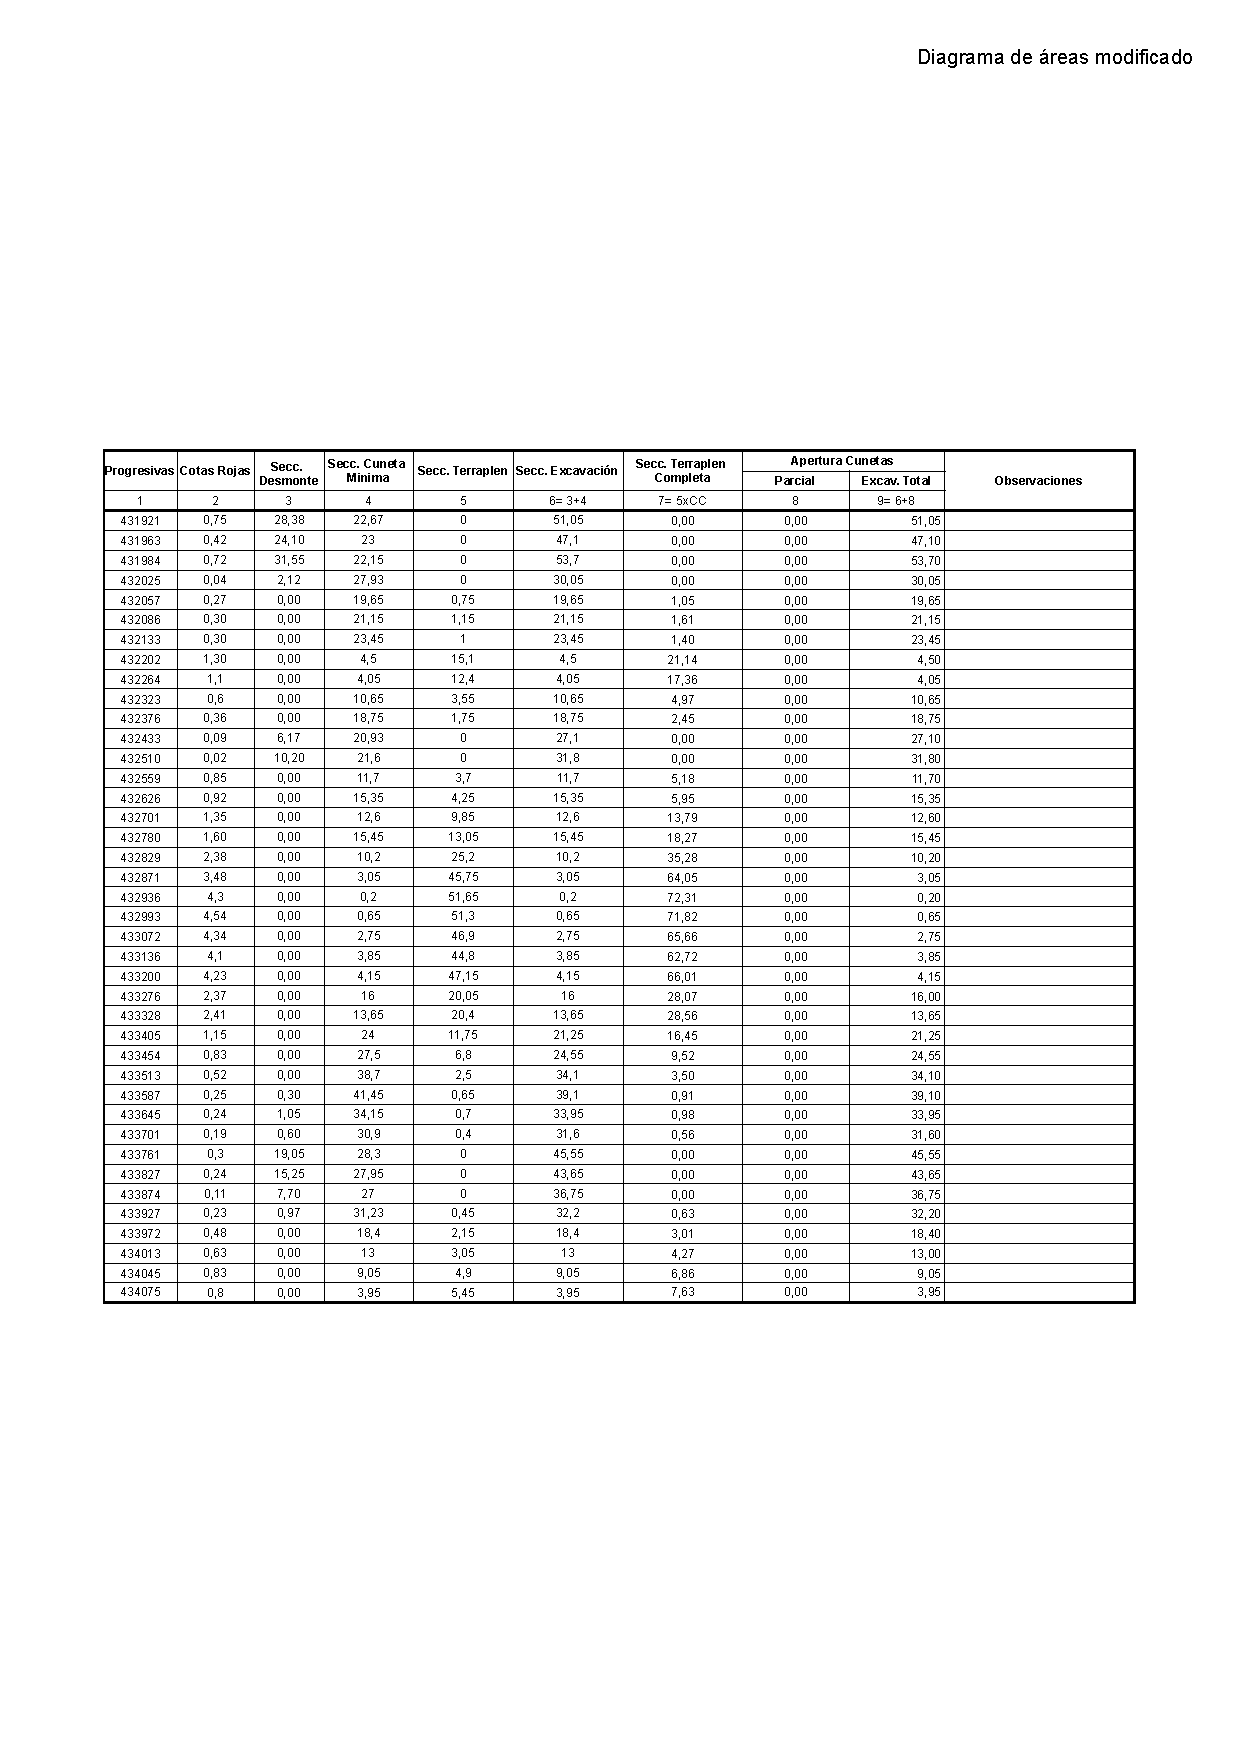
\includepdf[pages=-]{images/google_sheets/planilla_modificado.pdf}

\clearpage

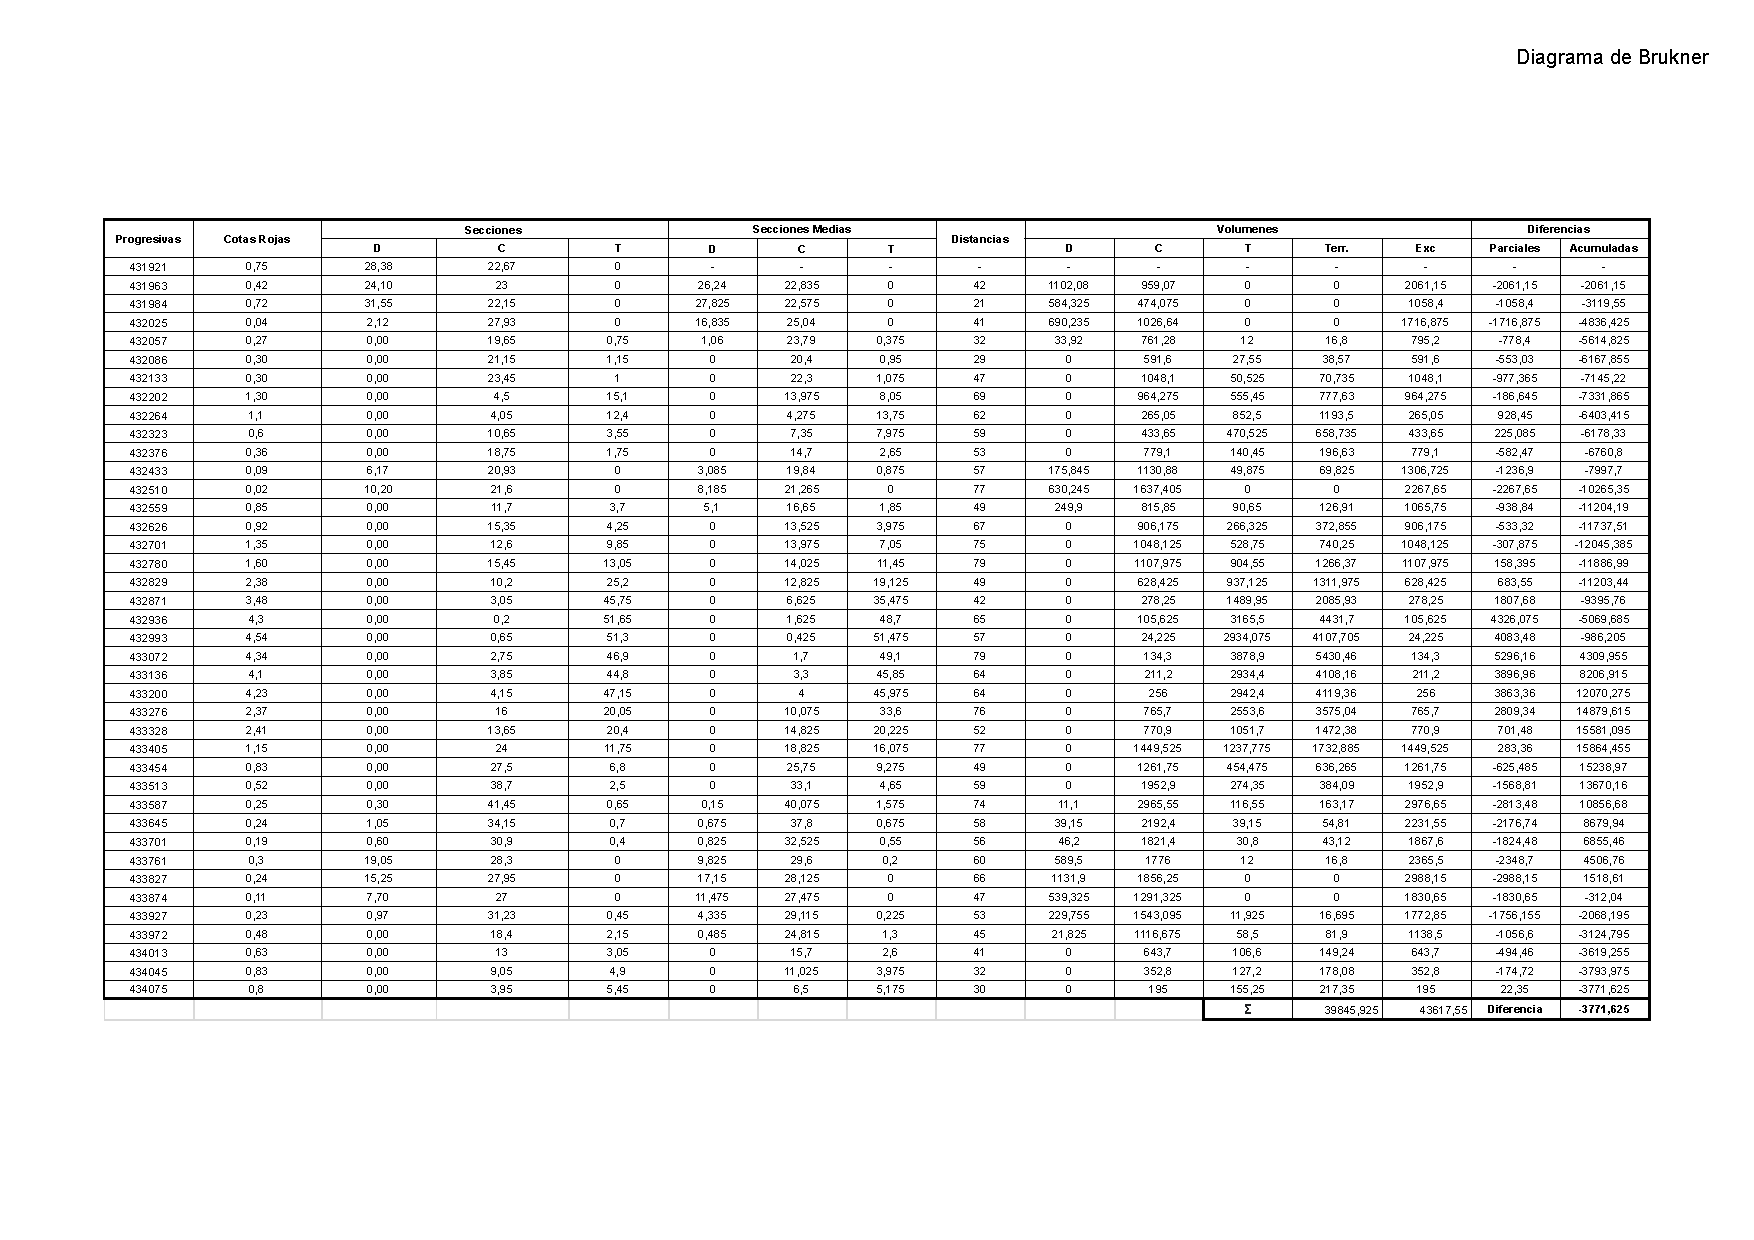
\includepdf[pages=-,angle=90]{images/google_sheets/planilla_bruckner.pdf}

\end{document}